\documentclass[11pt,a4paper,oneside]{report}

\usepackage{amsmath}
\usepackage{amsfonts}
\usepackage{amssymb}
\usepackage{graphicx}
\usepackage[top=2cm, bottom=2cm, left=3cm, right=2cm]{geometry}
\usepackage{a4wide}
\usepackage[english]{babel}
\usepackage[T1]{fontenc}
\usepackage{amsthm}
\usepackage{url}
\usepackage[utf8]{inputenc}
\usepackage[small,bf,hang]{caption}
\usepackage{fancyhdr}
\usepackage{float}
\usepackage[table]{xcolor}
\usepackage{hyphenat}
\usepackage{lscape}
\usepackage[square,numbers]{natbib}
\usepackage{hyperref}

% Custome Page Headers 
\pagestyle{fancy}
\fancyhf{}
\renewcommand{\headrulewidth}{0pt}
\fancyhf[HL]{\nouppercase{\textit{\leftmark}}}
\fancyhf[FC]{\thepage}

% Custom Paragraphs
\setlength{\parindent}{0pt}
\setlength{\headheight}{14pt}
\newcommand{\npar}{\par \vspace{2.3ex plus 0.3ex minus 0.3ex}}

\begin{document}

% Title details
\title{Software Architecture -- Phase I}
\author{Kristof Peeters \and Michiel Staessen}
\maketitle

% Table of Contents
\tableofcontents

% Content
\chapter{Domain Model}
\label{domain-model}

\chapter{Use Cases}
\label{use-cases}

\section{Use case diagram}

\npar The use case diagram is shown in figure \ref{fig:use-case-diagram}.

\begin{figure}[H]
	\begin{centering}
		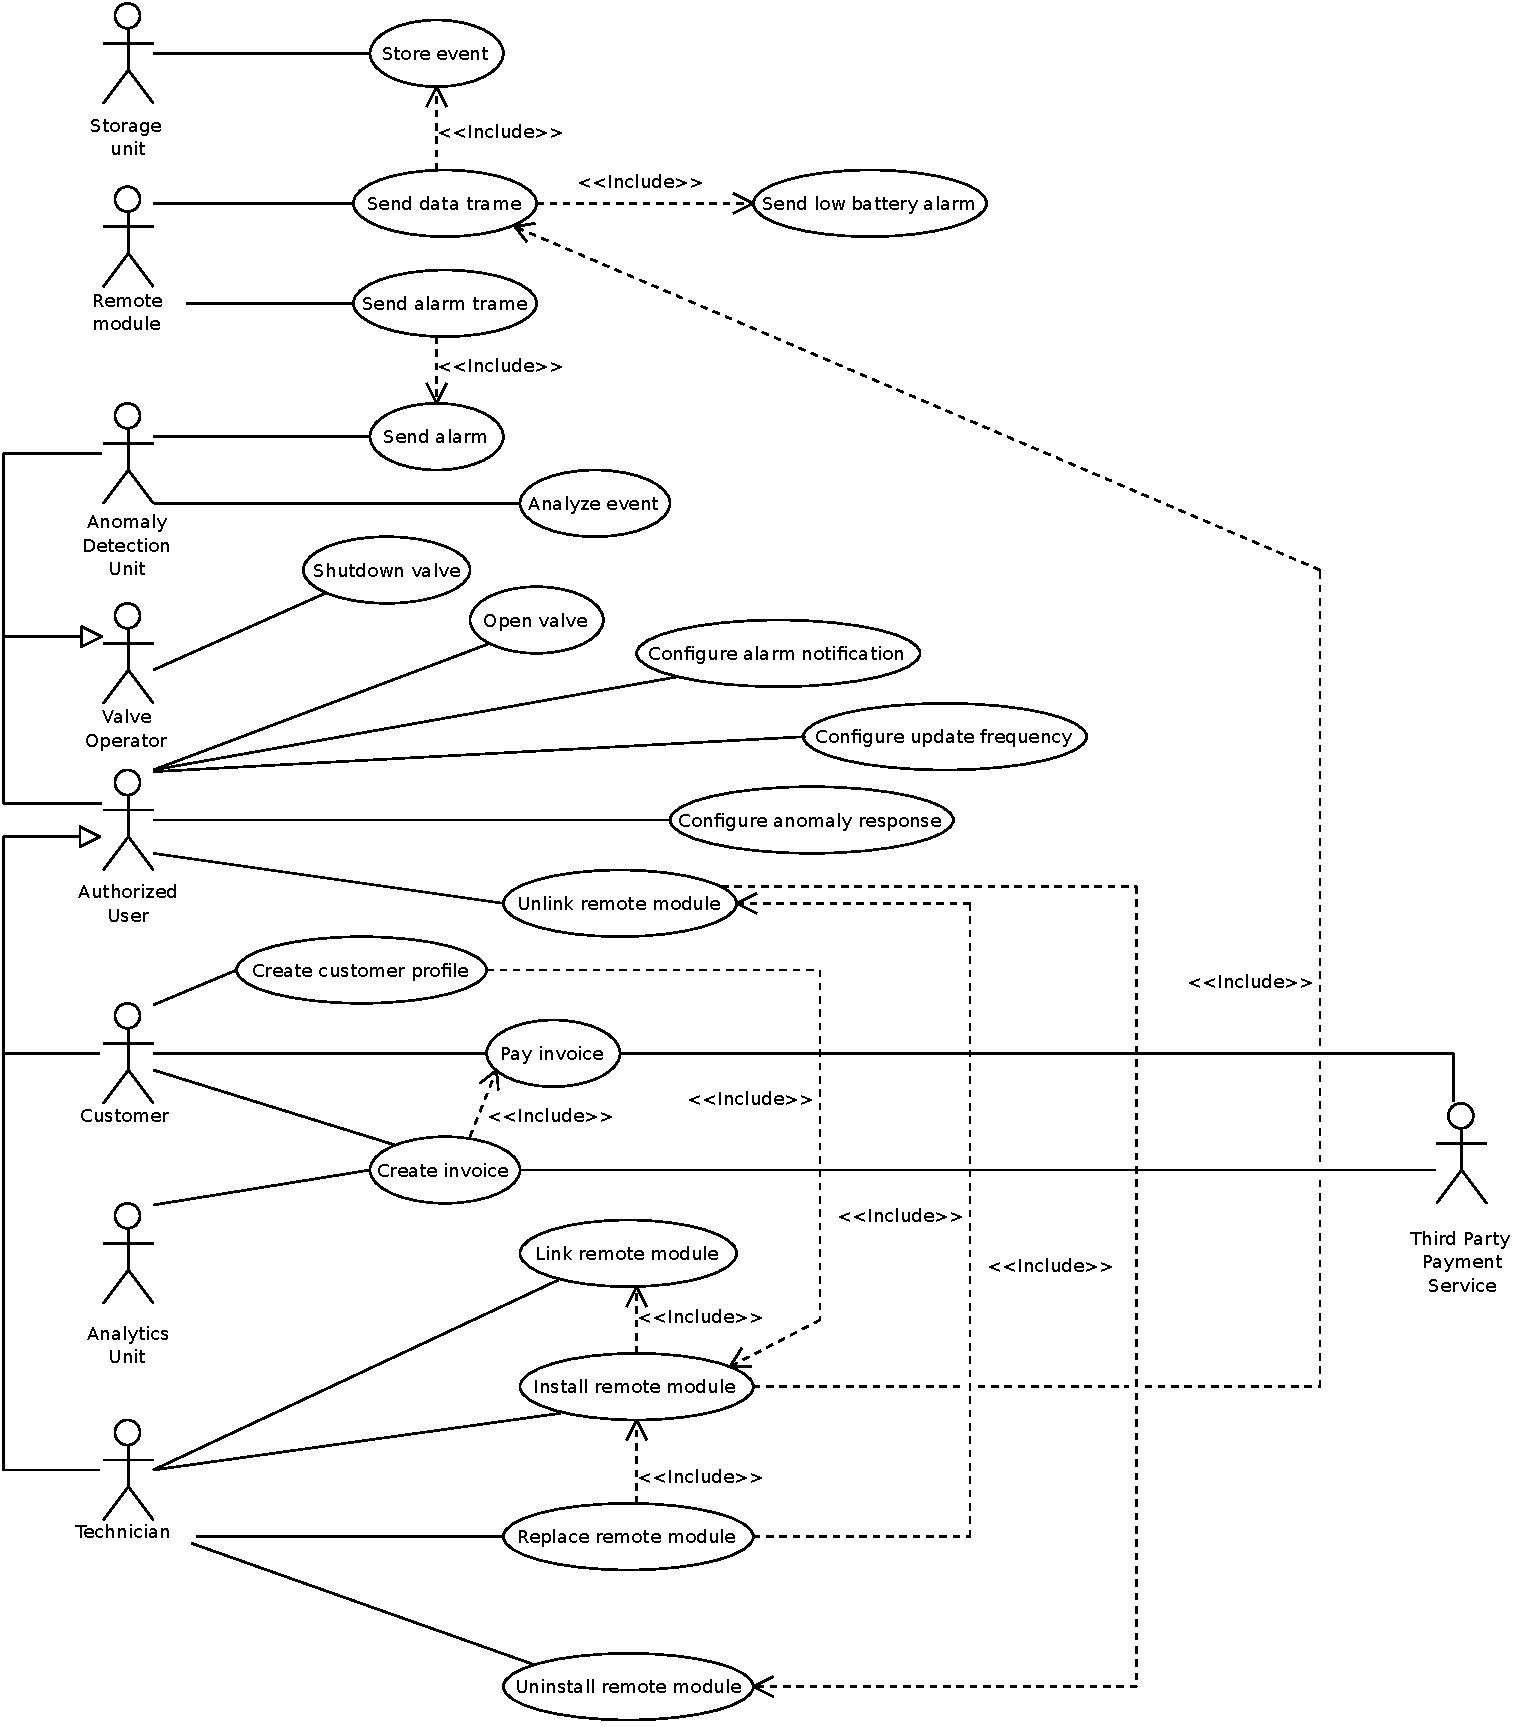
\includegraphics[width=\textwidth]{figs/use-case-diagram.pdf}
		\caption{Use case diagram}
		\label{fig:use-case-diagram}
	\end{centering}
\end{figure}

\section{Use cases}

\subsection{Create customer profile}
\label{uc:create-customer-profile}
\begin{description}
	\item[Primary actor] Customer
	\item[Interested parties] ReMeS, Utilty providing company, Call Center 
	\item[Preconditions] \ 
	\begin{itemize}
		\item The customer needs to have a contract on record with at least one
		utility providing company participating in the ReMeS program.
	\end{itemize}
	\item[Postconditions] \ 
	\begin{itemize}
		\item The customer has access to the ReMeS portal.
	\end{itemize}
	\item[Normal flow] \ 
	\begin{enumerate}
	  	% 1
		\item The customer contacts the ReMeS call center to request the necessary
		documents to be filled out.
		% 2
		\item A ReMeS employee operator sends the necessary documents to the
		residential user by regular mail.
		% 3
		\item The residential user fills out the required documents.
		% 4
		\item The customer sends the filled out forms back to ReMeS.
		% 5
		\item A ReMeS employee processes the customer's request and generates an
		authentication token (e.g. username and password)
		% 6
		\item A ReMeS employee sends an authentication token back to the residential
		user by regular mail.
	\end{enumerate}
	\item[Alternate flow] \ 
	\begin{description}
		\item[2a] The customer is a business/the customer has a business contract.
		\begin{enumerate}
			\item a ReMeS employee sends the necessary documents to the business owner.
			\item The alternate flow returns to step 3 in the normal flow.
		\end{enumerate}
		\item[6a] The customer is a business/the customer has a business contract.
		\begin{enumerate}
			\item a ReMeS employee sends the authentication token back to the business owner.
		\end{enumerate}
	\end{description}
	\item[Exception flow] \ 
	\begin{description}
		\item[5a] There are errors in the application.
		\begin{enumerate}
			\item a ReMeS employee sends the form back to the customer with addional
			information about the application not passing.
		\end{enumerate}
	\end{description}
\end{description}

\subsection{Link remote module}
\label{uc:link-remote-module}
\begin{description}
	\item[Primary actor] Technician
	\item[Interested parties] Customer, ReMeS, Utilty providing company, Call
	Center
	\item[Preconditions] \  
	\begin{itemize}
		\item The technician must be logged in into the ReMeS Portal.
		\item The customer needs to have a remote module installed.
		\item The remote module is registered in the ReMeS system.
	\end{itemize}
	\item[Postconditions] \ 
	\begin{itemize}
		\item The remote module is linked to the customer's profile.
	\end{itemize}
	\item[Normal flow] \ 
	\begin{enumerate}
	  	% 1
	  	\item The technician looks up the remote module profile.
	  	% 2 
	  	\item The technician looks up the customer's profile.
	  	% 3
	  	\item The technician connects the links the remote module profile to the
	  	customer's profile.
	  	% 4
	  	\item The technician confirms the link to be created between the two
	  	profiles.
	\end{enumerate}
\end{description}

\subsection{Unlink remote module}
\label{uc:unlink-remote-module}
\begin{description}
	\item[Primary actor] Authorized User
	\item[Interested parties] Customer, Technician, Call Center, Utility providing
	company
	\item[Preconditions] \ 
	\begin{itemize}
		\item The authorized user is logged in. 
		\item The remote module is registered.
		\item The remote module is activated.
	\end{itemize}
	\item[Postconditions] \ 
	\begin{itemize}
		\item The remote module is removed from the customer's profile.
		\item The remote module is removed from the customer's premise.
	\end{itemize}
	\item[Normal flow] \ 
	\begin{enumerate}
	  	% 1
	  	\item The authorized user indicates which remote module he or she
	  	wants to unlink.
	  	% 2
	  	\item The authorized user confirms the removal of the module from
	  	the customer's profile.
	  	% 3
	  	\item The authorized user schedules an appointment to uninstall the
	  	module.
		% 4
	  	\item At the scheduled appointment, include use case
	  	\ref{uc:uninstall-remote-module} (``Uninstall remote module'').
	\end{enumerate}
	\item[Exception flow] \
	\begin{description}
		\item[4a] The customer is not present at the scheduled appointment.
		\begin{enumerate}
			\item A call center operator contacts the customer to schedule a new
			appointment.
			\item Return to step 4 in the normal flow.
		\end{enumerate}
	\end{description}
\end{description}

\subsection{Install remote module}
\label{uc:install-remote-module}
\begin{description}
	\item[Primary actor] Technician
	\item[Interested parties] Customer, ReMeS, Utility providing company
	\item[Preconditions] \ 
	\begin{itemize}
	  	\item the customer needs to have an approved and activated customer profile
	  	in the ReMeS system.
	\end{itemize}
	\item[Postconditions] \ 
	\begin{itemize}
		\item The remote module is installed at the customer's premise.
		\item The remote module is activated.  
	\end{itemize}
	\item[Normal flow] \ 
	\begin{enumerate}
	  	% 1
		\item The technician arrives at the customer's premise.
		% 2
		\item The technician installs the module.
		% 3
		\item The technician registers the remote module with the ReMeS by entering
		the relevant information (e.g. serial number, brand, module type, location,
		initial meter value, other modules in front of this remote module, \ldots).
		% 4
		\item The technician configures the module for data communication.
		% 5
		\item The technician seals the module to prevent tampering.
		% 6
		\item The technician links the module to the customer's profile. Include use
		case \ref{uc:link-remote-module} (``Link remote module'').
		% 7
		\item The remote module sends its first trame, initializing the usage
		monitoring. Include use case \ref{uc:send-data-trame} (``Send data trame'').
	\end{enumerate}
\end{description}

\subsection{Uninstall remote module}
\label{uc:uninstall-remote-module}
\begin{description}
	\item[Primary actor] ReMeS
	\item[Interested parties] Customer, Utilty providing company
	\item[Preconditions] \ 
	\begin{itemize}
		\item ReMeS has at least one operating monitoring module.
	\end{itemize}
	\item[Postconditions] \ 
	\begin{itemize}
		\item The utility control module closes the valve in case a leak is detected.
		\item ReMeS is aware of this profile for the control module.
	\end{itemize}
	\item[Normal flow] \ 
	\begin{enumerate}
	  	% 1
	  	\item The user logs in to the ReMeS portal with his/her username and
	  	password.
	  	% 2
	  	\item The user navigates to the correct utility control module for
	  	reconfiguration.
	  	% 3 
	  	\item There he/she selects the profile on how to act in case a leak is
	  	detected. In this case, he/she chooses to immediately close the valve in
	  	case of leak.
	  	% 4
	  	\item ReMeS receives this reconfiguration request and sends the
	  	corresponding to command to the correct control module.
	  	% 5
	  	\item The module receives this command and acknowledges it.
	\end{enumerate}
	\item[Alternate flow] \ 
	\begin{description}
		\item
	\end{description}
	\item[Exception flow] \ 
	\begin{description}
		\item[1a] Username and/or password are wrong.
		\begin{enumerate}
		  \item correct the spellingserrors(s) and retry.
		\end{enumerate}
		\item[4a] The request is lost.
		\begin{enumerate}
		  \item The user portal doesn't get an acknowledgement and has to resend the
		  request.
		\end{enumerate}
		\item[5a] The command is lost or not executed.
		\begin{enumerate}
		  \item The ReMeS system doesn't get an acknowledgement and has to resend the
		  command.
		 \end{enumerate}
	\end{description}
\end{description}

\subsection{Replace remote module}
\label{uc:replace-remote-module}
\begin{description}
	\item[Primary actor] Technician
	\item[Interested parties] Customer, ReMeS, Utility providing company
	\item[Preconditions] \ 
	\begin{itemize}
		\item The customer has a faulty or outdated remote module installed.
	\end{itemize}
	\item[Postconditions] \ 
	\begin{itemize}
		\item The remote module is replaced.
		\item The new remote module is installed, registered and activated. 
	\end{itemize}
	\item[Normal flow] \ 
	\begin{enumerate}
	  	% 1
	  	\item The technician arrives at the customer's premise;
	  	% 2
	  	\item The technician unlinks and uninstalls the module. Include use case
	  	\ref{uc:unlink-remote-module} (``Unlink Remote module'').
	  	% 3
	  	\item The technician installs and links the new module. Include use case
	  	\ref{uc:install-remote-module} (``Install remote module''). 
	  	% 4
	  	\item The technician leaves.
	\end{enumerate}
\end{description}

\subsection{Configure transmission frequency}
\label{uc:configure-transmission-frequency}
\begin{description}
	\item[Primary actor] Authorized user
	\item[Interested parties] Customer, ReMeS, Utility providing company
	\item[Preconditions] \ 
	\begin{itemize}
		\item The authorized user is logged into the ReMeS portal.
		\item The customer has an installed, registered and active monitoring module.
	\end{itemize}
	\item[Postconditions] \ 
	\begin{itemize}
		\item The update frequency of the module has changed.
	\end{itemize}
	\item[Normal flow] \ 
	\begin{enumerate}
	  	% 1
	  	\item The authorized user indicates for which module he wants to reconfigure
	  	the update frequency.
	  	% 2 
	  	\item The authorized user changes the update frequency for the monitoring
	  	module module.
	  	% 3
	  	\item The authorized user confirms the update frequency changes.
	  	% 4
	  	\item The communication unit sends the reconfiguration request to the
	  	correct remote module.
	  	% 5
	  	\item The remote module receives the request.
	  	% 6
	  	\item The remote module reconfigures itself.
	  	% 7
	  	\item The remote module acknowledges the change if successful.
	\end{enumerate}
	\item[Exception flow] \ 
	\begin{description}
		\item[5a] The remote does not receive the request.
		\begin{enumerate}
			\item The communication unit waits for a while.
			\item Return to step 4 of the normal flow.
		\end{enumerate}
		\item[6a] Reconfiguration fails.
		\begin{enumerate}
			\item The remote module keeps the old setting.
			\item An error message will be displayed on the ReMeS portal.
			\item The use case ends here.
		 \end{enumerate}
	\end{description}
\end{description}

\subsection{Configure alarm notification}
\label{uc:configure-alarm-notification}
\begin{description}
	\item[Primary actor] Customer
	\item[Interested parties] ReMeS, Utilty providing company
	\item[Preconditions] \ 
	\begin{itemize}
		\item The customer is registered in the ReMeS system.
	\end{itemize}
	\item[Postconditions] \ 
	\begin{itemize}
		\item The new alarm configuration is stored.
	\end{itemize}
	\item[Normal flow] \ 
	\begin{enumerate}
	  	% 1
	  	\item The user logs in to the ReMeS portal with his/her username and
	  	password.
	  	% 2
	  	\item The user navigates to the correct module for alarm
	  	notification recipient configuration.
	  	% 3 
	  	\item There he/she adds the required contact details, namely email address
	  	and (mobile) phone number.
	  	% 4
	  	\item System acknowledges the received details.
	\end{enumerate}
	\item[Alternate flow] \ 
	\begin{description}
		\item
	\end{description}
	\item[Exception flow] \ 
	\begin{description}
		\item[1a] Username and/or password are wrong.
		\begin{enumerate}
		  \item correct the spellingserrors(s) and retry. %TODO return
		\end{enumerate}
		\item[4a] One or more of the contact details are incorrect. (for example an
		email address without a domain name)
		\begin{enumerate}
		  \item The user is notified and has to correct the incorrect details.
		\end{enumerate}
	\end{description}
\end{description}

\subsection{Configure anomaly response}
\label{uc:configure-anomaly-response}
\begin{description}
	\item[Primary actor] Customer
	\item[Interested parties] ReMeS, Utilty providing company
	\item[Preconditions] \ 
	\begin{itemize}
		\item The customer is logged in into the ReMeS portal.
		\item The customer has a remote valve installed.
		\item The remote valve is active and registered in the ReMeS system.
	\end{itemize}
	\item[Postconditions] \ 
	\begin{itemize}
		\item The new alarm configuration is stored.
	\end{itemize}
	\item[Normal flow] \ 
	\begin{enumerate}
	  	% 1
	  	\item The customer indicates for which remote valve he or she wants to
	  	(re)configure the anomaly detection response.
	  	% 2
	  	\item The customer sets the desired anomaly detection response (shut down
	  	automatically, delayed shut down, no shut down).
	  	% 3
	  	\item The customer confirms the new anomaly detection response.
	\end{enumerate}
\end{description}

\subsection{Send data trame}
\label{uc:send-data-trame}
\begin{description}
	\item[Primary actor] Remote module
	\item[Interested parties] Customer, Utility providing company, ReMeS
	\item[Preconditions] \ 
	\begin{itemize}
		\item The remote module is installed.
		\item The remote module is activated.
	\end{itemize}
	\item[Postconditions] \ 
	\begin{itemize}
		\item The data center has collected a trame.
	\end{itemize}
	\item[Normal flow] \ 
	\begin{enumerate}
	  	% 1
		\item The remote module prepares a data trame with all the information (date
		and time, battery level, counter values, \ldots).
		% 2
		\item The remote module sends the trame to the configured phone number by SMS.
		% 3
		\item The data center collects the trame.
		% 4
		\item The data center processes the trame.
	\end{enumerate}
	\item[Alternate flow] \ 
	\begin{description}
		\item[2a] The remote module uses the internet to send trames.
		\begin{enumerate}
			\item The remote module sends the trame to the configured IP address using
			the configured WiFi connection.
			\item Return to step 3 in the normal flow.
		\end{enumerate}
		\item[4a] The battery is low.
		\begin{enumerate}
			\item Include Use Case \ref{uc-low-battery-alarm} (``Low Battery Alarm'').
		\end{enumerate}
	\end{description}
	\item[Exception flow] \ 
	\begin{description}
		\item[2a] The trame cannot be sent (timeout or wrong response code).
		\begin{enumerate}
			\item The remote module waits for 5 minutes;
			\item Return to step 1 in the normal flow.  
		\end{enumerate}
	\end{description}
\end{description}

\subsection{Send alarm trame}
\label{uc:send-alarm-trame}
\begin{description}
	\item[Primary actor] Remote monitoring module
	\item[Interested parties] Customer, Call Center, Utility providing company,
	ReMeS, Emergency services
	\item[Preconditions] \ 
	\begin{itemize}
	  	\item An anomaly detection algorithm triggered the alarm.
		\item The remote module is installed and active.
		\item The customer needs to have an alarm configuration.
	\end{itemize}
	\item[Postconditions] \ 
	\begin{itemize}
		\item The event is logged.
		\item The consumption profile is updated.
	\end{itemize}
	\item[Normal flow] \ 
	\begin{enumerate}
	  	% 1
	  	\item The remote monitoring module prepares an alarm trame.
	  	% 2
	  	\item The remote monitoring module sends the alarm trame to the configured
	  	data center. 
	  	% 3 
	  	\item The data center collects the alarm trame.
		% 4
		\item The data center converts the alarm trame to an alarm event.
		% 5
		\item The storage unit saves the alarm event.
		% 6
	  	\item The anomaly detection unit examines the alarm event.
		% 7
	  	\item The anomaly detection unit sends a notification to the customer.
	  	Include use case \ref{uc-alarm-transmission-remes} (``Alarm transmission: ReMeS'').
	\end{enumerate}
	\item[Alternate flow] \ 
	\begin{description}
		\item[4a] The trame is coming from a remote gas monitoring module.
			\begin{enumerate}
				\item ReMeS sends a shutdown command to the remote valve.
				\item The remote valve shuts down.
				\item The remote valve acknowledges to ReMeS if the shutdown was successful.
			\end{enumerate}
		\item[6a] The data center recognizes this alarm trame as a false alarm.
		\begin{enumerate}
			\item ReMeS records a false alarm.
			\item The use case ends here. 
		\end{enumerate}
	\end{description}
	\item[Exception flow] \ 
	\begin{description}
		\item[2a] The trame could not been sent. 
		\begin{enumerate}
			\item The remote module waits for 3 seconds.
			\item Return to step 2 of the normal flow.
		\end{enumerate}
	\end{description}
\end{description}

\subsection{Send alarm}
\label{uc:send-alarm}
\begin{description}
	\item[Primary actor] ReMeS
	\item[Interested parties] Customer, Call Center, Utility providing company,
	Emergency services
	\item[Preconditions] \ 
	\begin{itemize}
		\item The customer needs to have an alarm configuration registrerd in ReMeS.
		\item ReMeS has detected an anomaly in the consumption pattern of a
		customer OR an alarm has been sent from a remote monitoring module.
	\end{itemize}
	\item[Postconditions] \ 
	\begin{itemize}
		\item The event is logged.
		\item The consumption profile is updated.
	\end{itemize}
	\item[Normal flow] \ 
	\begin{enumerate}
	  	% 1
	  	\item ReMeS sends either an email or a text message (depending on
	  	the configuration) to notify the customer that there is a potential anomaly.
	  	% 2 
	  	\item The customer receives the email or sms and reads it.
		% 3
	  	\item The customer determines that is indeed an anomaly.
		% 4
	  	\item The customer logs in into the ReMeS portal and indicates that the detected anomaly was indeed an anomaly.
	\end{enumerate}
	\item[Alternate flow] \ 
	\begin{description}
		\item[4a] The reported alarm is a falsa alarm.
		\begin{enumerate}
		  \item The customer logs in into the ReMeS portal and indicates that the detected anomaly was a false alarm.
		\end{enumerate}
	\end{description}
	\item[Exception flow] \ 
	\begin{description}
		\item[2a] The alarm message can not be sent.
		\begin{itemize}
			\item ReMeS waits for 3 seconds.
			\item Return to step 2 in Normal flow. 
		\end{itemize}
	\end{description}
\end{description}

\subsection{Send low battery alarm}
\label{uc:send-low-battery-alarm}
\begin{description}
	\item[Primary actor] Remote module
	\item[Interested parties] Customer, Utility providing company, ReMeS
	\item[Preconditions] \ 
	\begin{itemize}
		\item A trame is collected
		\item The battery status of the collected trame indicates that the battery is
		indeed low.
		\item The trame comes from a battery powered module.
	\end{itemize}
	\item[Postconditions] \ 
	\begin{itemize}
		\item The battery in the remote module is replaced. 
	\end{itemize}
	\item[Normal flow] \ 
	\begin{enumerate}
	  	% 1
	  	\item The ReMeS sytems sends out an alarm to the designated customer using a
	  	user-defined alarm configuration.
	  	% 2
		\item The customer responds to the alarm notification by replacing the
		battery.
	\end{enumerate}
	\item[Alternate flow] \ 
	\begin{description}
		\item[1a] An alarm is already sent in the last 24 hours.
		\begin{enumerate}
			\item ReMeS waits until 24 hours since the last alarm have passed.
		\end{enumerate}
		\item[1b] Multiple alarms (10) have been sent and the customer is not
		responding.
		\begin{enumerate}
			\item ReMeS dispatches a technician.
			\item The technician replaces the battery.
		\end{enumerate}
		\item[2a] The customer responds to the alarm by notifying the ReMeS call
		center to inform ReMeS the customer is not able to replace the battery. 
		\begin{enumerate}
			\item ReMeS dispatches a technician.
			\item The technician replaces the battery.
		\end{enumerate}
	\end{description}
\end{description}

\subsection{Close valve}
\label{uc:close-valve}
\begin{description}
	\item[Primary actor] Valve Operator
	\item[Interested parties] Customer, ReMeS, Utility providing company
	\item[Preconditions] \ 
	\begin{itemize}
		\item The remote valve is installed at the customer's premise.
		\item The remote valve is registered.
		\item The remote valve is active.
		\item The remote valve is open.
		\item A request has been made to shut down the valve.
	\end{itemize}
	\item[Postconditions] \ 
	\begin{itemize}
		\item The valve is shut down.
	\end{itemize}
	\item[Normal flow] \ 
	\begin{enumerate}
	  	% 1
	  	\item The valve operator indicates which remote valve needs to be shut down.
	  	% 2 
	  	\item The communication unit sends a request to the remote valve to shut it
	  	down.
	  	% 3
	  	\item The remote valve shuts down.
	  	% 4
	  	\item The remote valve notifies the communication unit in case the
	  	shutdown is successful.
	\end{enumerate}
	\item[Exception flow] \ 
	\begin{description}
		\item[2a] The communication unit cannot reach the remote valve.
		\begin{enumerate}
		  \item The communication unit waits till the module calls the base.
		  \item Return to step 2 in normal flow.
		\end{enumerate}
		\item[4a] The acknowledgement times out.
		\begin{enumerate}
			\item The remote module tries again for up to three times.
		\end{enumerate}
	\end{description}
\end{description}

\subsection{Create invoice}
\label{uc:create-invoice}
\begin{description}
	\item[Primary actor] AnalyticsUnit
	\item[Interested parties] Customer, Utility providing company, Third Party
	Payment Service
	\item[Preconditions] \ 
	\begin{itemize}
		\item The customer needs to be registrered in the ReMeS system.
	\end{itemize}
	\item[Postconditions] \ 
	\begin{itemize}
		\item The customer now has a pending invoice.
		\item The utility providing company and third party payment service receive a
		copy of the invoice.
	\end{itemize}
	\item[Normal flow] \ 
	\begin{enumerate}
	  	% 1
	  	\item The system generates the usage detail for a certain period of time.
	  	% 2
	  	\item Using the information in the contract between the utility providing
	  	company and the customer, the system calculates the total price for the
	  	consumption.
	  	% 3 
	  	\item This amount, together with the start and end date of the period, makes
	  	up the invoice.
	  	% 4  
	  	\item Then the invoice is dispatched to the third party payment
	  	service and the utility providing company. This could be either electronicly
	  	or by regular mail.
	\end{enumerate}
	\item[Alternate flow] \ 
	\begin{description}
		\item 
	\end{description}
	\item[Exception flow] \ 
	\begin{description}
		\item 
	\end{description}
\end{description}

\subsection{Pay invoice}
\label{uc:pay-invoice}
\begin{description}
	\item[Primary actor] Customer
	\item[Interested parties] ReMeS, Utility providing company, Third Party Paymeny
	Service
	\item[Preconditions] \ 
	\begin{itemize}
		\item The customer has a pending invoice.
		\item The third party payment service has the invoice at it's disposal.
	\end{itemize}
	\item[Postconditions] \ 
	\begin{itemize}
		\item The customer has no more pending invoices and the invoice is paid.
		\item The utility providing company and third party payment service each got
		their share of the paid invoice.
	\end{itemize}
	\item[Normal flow] \ 
	\begin{enumerate}
	  	% 1
	  	\item The third party payment service notifies the customer that there is a
	  	pending invoice
	  	% 2
	  	\item The customer transfer the correct amount of money to the payment
	  	service before expiration of the due date.
	  	% 3 
	  	\item Upon receiving the correct amount of money from the customer, the
	  	payment service notifies ReMeS and the corresponding utility providing
	  	company.
	\end{enumerate}
	\item[Alternate flow] \ 
	\begin{description}
		\item[2a] The customer does not pay on time
		\begin{enumerate}
		  \item a last warning to pay is sent.
		  \item 
		\end{enumerate}
	\end{description}
	\item[Exception flow] \ 
	\begin{description}
		\item 
	\end{description}
\end{description}

\chapter{Additional constraints}
\label{additional-constraints}

\begin{itemize}
	\item A utility providing company can only manage modules for the utilities it
	provides.
	\item The customer of every event is equal to the customer that belongs to the
	remote module that sent the trame, resulting in the generation of the event.
	\item Modules that depend on each other (monitor/valve combinations, multiple
	monitoring modules on the same line, \ldots) should always concern the same
	utility.
	\item WiFiModules should always use an external power because the WiFi.
	connection consumes to much electricity.
	\item Only battery powered modules can send low battery alarms.
	\item The update frequency on battery powered devices can only be once per 24 hours. 
	\item The cumulative values of subsequent measurements of a remote
	monitoring module should rise monotonically except when the monitoring module
	is installed on a utility that can supply to the grid (e.g. houses with solar
	energy).
	\item No access is granted to the ReMeS portal without authentication.
	\item No access to personal data in the ReMeS portal is allowed without
	authorization.
	\item No valves should be shut without a previous anomaly detection.
	\item No alarms should be triggered without a anomaly detection.
	\item In case of a gas leak, the customer and the emergency services should be
	notified.
	\item In case of a water leak, only the customer should be notified.
	\item A customer cannot receive invoices from a utility providing company with
	whom the customer has no contract.
	\item In order to create a user profile for ReMeS, the utility company should
	participate in the ReMeS program.
\end{itemize}
\chapter{Quality attribute scenario's}
\label{quality-attribute-scenarios}

\section{Availability}

\subsection{Remote module}
\label{qas-av-module}
\begin{description}
	\item[Source] Internal to the system
	\item[Stimulus] Fault: due to a hardware failure, the software stops working.
	\item[Artifact] Remote module 
	\item[Environment] During normal operation 
	\item[Response] \ %TODO: SLA met hardware manufacturer vermelden ?
	\begin{enumerate}
	  \item The system should detect and record the event.
	  \item As long as the corresponding module is not repaired, no data can
	  be received from or send to this module.
	  \item The module's host (i.e. the customer where the module is hosted) should
	  be notified.
	  \item A specialized technician should be dispatched to repair or replace the
	  module.
	\end{enumerate}
	\item[Response measure] \ 
	\begin{enumerate}
	  \item The detection time should be at most the update frequency of the
	  corresponding module.
	  \item In 98\% of all cases the problem should be fixed within 2 days.
	  \item If these problems occur systematicly (rate > 2/year), usage
	  analysis and revision of SLA should be done within one month.
	\end{enumerate}
\end{description}

\subsection{Network}
\label{qas-av-network}
\begin{description}
	\item[Source] External to the system
	\item[Stimulus] Fault: The transmission of data is unexpectedly
	(i.e. not by a scheduled maintenance) interrupted.
	\item[Artifact] Communication channels
	\item[Environment] During normal operation
	\item[Response] \
	\begin{enumerate}
	  \item The system should detect the network failure.
	  \item During the breakdown, no additional measurements can be collected nor
	  can alarms from modules be received. 
	  \item To prevent a (useless) overreaction, some basic troubleshooting is
	  passed through (checking the physical connections, rebooting the router,
	  etc.).
	  \item In case none of the above basic tips solved the problem, the network
	  provider should be notified about the crash.
	\end{enumerate}
	\item[Response measure] \
	\begin{enumerate}
	  \item Detection should be done under 1 minute.
	  \item In accordance to the SLA with the telecom operator, the data flow
	  should be re-established within the specified period.
	  \item If these problems occur systematicly (rate > 1/month), usage
	  analysis and revision of SLA should be done within one month.
	\end{enumerate}
\end{description}

\subsection{Data center}
\label{qas-av-datacenter}
\begin{description}
	\item[Source] Internal to the system
	\item[Stimulus] Hardware failure in the datacenter. Since the datacenter
	consists of several units, there could be various reasons for failure: one of
	the analysis, prediction, anomaly detection or storage servers goes down.
	\item[Artifact] All of the entities which make up the datacenter could be the
	artifact :
	\begin{enumerate}
	  \item Analysis unit
	  \item Prediction unit
	  \item Anomaly detection unit
	  \item Storage unit
	\end{enumerate}
	\item[Environment] During normal operation
	\item[Response] \
	\begin{enumerate}
	  \item Independent of the unit that goes down, the system should detect the
	  crash.
	  \item If the analysis or prediction unit goes down:
	  \begin{enumerate}
	    \item Any pending operations on the server should be cancelled and those
	    temporary results are lost (i.e. they have to be recalculated).
	    \item As long as the server is down, no new advices, predictions or alarms
	    can be made.
	    \item Under no circumstances can this failure leave (or bring) the system
	    in an inconsistent state.
	    \item A technician is dispatched to resolve the problem, this could be a
	    replacement of one single component or the whole server. The technician
	    could be belonging to ReMeS or the hardware manufacturer.
	    \item Upon resolving the problem, the server can resume his analysis,
	    prediction or anomaly detection tasks.
	  \end{enumerate}
	  \item If the storage unit goes down:
	  \begin{enumerate}
	   \item There should be at least one replica of all the data because ReMeS
	   core business (i.e. predicting, monitoring and analyzing) all relies on
	   (available) data.
	   \item Any pending operations on this (crashed) server should be cancelled
	   and resumed or restarted on the replica. In this way the rest of the system
	   has no knowledge of this recent crash.
	   \item Under no circumstances can this failure leave (or bring) the system
	    in an inconsistent state.
	    \item A technician is dispatched to resolve the problem, this could be a
	    replacement of one single component or the whole server. The technician
	    could be belonging to ReMeS or the hardware manufacturer.
	    \item When the main server is back up and running, the replica can return
	    control to the main server.
	  \end{enumerate}
	\end{enumerate}
	\item[Response measure] \
	\begin{enumerate}
	  \item The system has a guaranteed uptime of 99.9\% excluded from scheduled
	  maintenance.
	  \item In accordance to the SLA with the hardware manufacturer, the hardware
	  is repaired or replaced on time with respect to the SLA.
	\end{enumerate}
\end{description}

\section{Performance}

\subsection{Gas leak}
\label{qas-perf-gas}
\begin{description}
	\item[Source] Gas monitoring module, Internal to the system.
	\item[Stimulus] Gas leak alarm message.
	\item[Artifact] System.
	\item[Environment] During normal mode.
	\item[Response] \
		\begin{enumerate}
		  \item The system should record the message
		  \item Upon processing the message, the customers who could experience
		  inconvenience are notified.
		  \item The emergency services (i.e. the fire department) are dispatched.
		  \item All control modules in the neighbourhood of the leak are sealed off in
		  any case.
		\end{enumerate}
	\item[Response measure] 
	\begin{enumerate}
	  \item 95\% of all notifications should reach the recipient in 30s. 
	  \item %TODO: upper limit on closure of the valves ?
	\end{enumerate}
\end{description}

\subsection{Water leak}
\label{qas-perf-water}
\begin{description}
	\item[Source] Gas monitoring module, Internal to the system.
	\item[Stimulus] Gas leak alarm message.
	\item[Artifact] System.
	\item[Environment] During normal mode.
	\item[Response] \
		\begin{enumerate}
		  \item The system should record the message
		  \item Upon processing the message, the customers who could experience
		  inconvenience are notified.
		  \item The emergency services (i.e. the fire department) are dispatched.
		  \item All control modules in the neighbourhood of the leak are sealed off in
		  any case.
		\end{enumerate}
	\item[Response measure] 
	\begin{enumerate}
	  \item 95\% of all notifications should reach the recipient in 30s. 
	  \item %TODO: upper limit on closure of the valves ?
	\end{enumerate}
\end{description}

\subsection{??}
\label{qas-perf-other}
\begin{description}
	\item[Source] Battery-powered module
	\item[Stimulus] Low battery alarm
	\item[Artifact] System
	\item[Environment] During normal mode 
	\item[Response] \
	\begin{enumerate}
	  \item ReMeS sends a notification to the customer.
	  \item Customer replaces the battery or if the customer is not capable of
	  doing so then a ReMeS technician will be dispatched to solve the problem.
	\end{enumerate}
	\item[Response measure] \
	\begin{enumerate}
	  \item 98\% of all the batteries should be replaced before the corresponding
	  modules stop sending trames.
	\end{enumerate}
\end{description}
\chapter{Glossary}
\label{chap:glossary}

\begin{description}
\item[Advice] An \emph{advice} is information provided to the customer in order
to reduce one's \emph{utility} bill. This information is typically obtained through
analysis of one's consumption.

\item[Alarm] An \emph{Alarm} is a message sent by ReMeS to inform the customer
that some anomaly is detected. This could be e.g. an excessive usage of a cetrain
\emph{utility}.

\item[AlarmCall] An \emph{AlarmCall} represents the telephone conversation
between ReMeS and the \emph{Customer}.

\item[AlarmConfiguration] An \emph{AlarmConfiguration} is a general name for the
contact details of a \emph{customer}. \emph{Customers} can be reached via sms or
email.

\item[AlarmEvent] An \emph{AlarmEvent} is an event which is sent from the
\emph{CommunicationUnit} to the \emph{DataCenter} when the latter receives an
\emph{AlarmTrame}. This is a single format that every unit of the
\emph{DataCenter} can read.

\item[AlarmTrame] This is a \emph{Trame} send by a \emph{module} to report an
\emph{alarm}. This could be in any format, depending on the \emph{module}.

\item[AnalysticsUnit] The \emph{AnalyticsUnit} is responsible for the analysis
of all the monitoring data originating from the \emph{customers}. This analysis
includes several algorithms to generate detailed consumption patterns,
\emph{advices} and \emph{reports}. 

\item[AnomalyDectectionUnit] The \emph{AnomalyDectectionUnit} runs several
Machine Learning algorithms to detect leaks and other anomalies. Furthermore any
\emph{alarms} generated by \emph{modules} are passed to this unit so it can take
appropriate steps (i.e. generate an \emph{alarm}).

\item[Authorized User] An \emph{Authorized User} is a user that can make changes
in the ReMeS system on behalf of other customers (e.g. a Technician) or on
behalf of itself (e.g. the customer). %TODO

\item[BoughtModule] The \emph{boughtModule} refers to \emph{modules} which are
bought by utility companies when they decide to not outsource the billing aspect
to ReMeS.

\item[BusinessCustomer] A \emph{BusinessCustomer} is a company which is a
\emph{customer} (of ReMes and/or several utility companies). The company is a
consumer of \emph{utilities} and so not necessarily a utility company itself.

\item[CallCenter] This is the contact center for troubleshooting and notifying
customers. \emph{Alarms} which are 

\item[Company] A \emph{Company} is in the context of this project a
\emph{utility} company. A \emph{Company} can provide more than \emph{utility}. 

\item[CommunicationUnit] This unit is responsible for the collection of data
from all the \emph{modules}. Data could be in different formats (dependent on
the \emph{module}) and could be received through various communication media.

\item[Contract] A Contract is negotiated between a \emph{Customer} and a
\emph{Company} and connects both parties inextricable for a certain period of
time. When one of the two parties wishes to terminate this \emph{Contract}
premature, they typically will have to have a valid reason also included in the
\emph{Contract}. Furthermore there is typically information included about the
price per unit per utility.

\item[Configuration] A \emph{Configuration} denotes the tuning of a
\emph{module}. This could e.g. the automatic closure of valves in case of an
anomaly.

\item[Customer] A \emph{Customer} is a recipient of a \emph{utility} in exchange
for a payment based on the his/her or it's consumption. There are two kinds of
\emph{Customers}: \emph{ResidentialCustomers} \emph{BusinessCustomers}.

\item[DataCenter] \emph{DataCenter} is a general name for all the different
units in the system. This is a clever notation to easily refer to AnalyticsUnit,
PredictionUnit, StorageUnit and AnomalyDetectionUnit in one time.

\item[Electricity] \emph{Electricity} is used in this context as the public
service, \emph{Electricity}.

\item[EmergencyCall] An \emph{EmergencyCall} is special kind of
\emph{AlarmCall}, namely to the \emph{EmergencyService}.

\item[EmergencyService] Emergency services are organizations which ensure public
safety and health by addressing different emergencies. The three main services
are: Police, Fire Department and Medical urgency.

\item[Event] An event is a message which is send from the
\emph{CommunicationUnit} to one of the units of the \emph{DataCenter} (it is a
one-way traffic message, so it is not send in the other direction). It forms a
generalisation for \emph{UpdateEvents} and \emph{AlarmEvents}.

\item[Gas] \emph{Gas} is used in this context as the public service,
\emph{Gas}.

\item[Government] The \emph{Government} is a stakeholder of ReMeS with as main
concern having insight in the usage statistics of utilities in the country.
Foreign \emph{governmnent} are also stakeholders if \emph{utilities} are
exported or imported.

\item[GPRSModule] This refers to a specific kind of \emph{Module} which
communicates with the \emph{CommunicationUnit} through the use of GPRS
technology.

\item[HiredModule] A \emph{HiredModule} is a \emph{Module} hired by a
\emph{customer}. This occurs when a \emph{company} has outsourced the billing
aspect to ReMeS.

\item[Invoice] An Invoice is a document containing the consumption of a
\emph{Customer} for a certain utility during a certain period of time.
Furthermore (and more important), this document also contains the total amount
the \emph{Customer} has to pay for this consumption to the \emph{Company}.

\item[IPCommunicationUnit] This unit is responsible for the collection of
measurement data through GPRS and Wifi. The collected data is then send to the
DataCenter.

\item[Module] This is a general name for all sorts of modules.
There are \emph{Modules} who measure monitor data and \emph{Modules} that can
control the flow (valves). Another way in which \emph{Modules} can differ is the
communication type (i.e. GPRS, SMS and Wifi). A final distinction is the owner,
modules can be owned by a \emph{Company} or hired by a customer.

\item[MonitoringModule] This is a \emph{Module} which measures the consumption
of a certain \emph{utility}. The measured data is send to the
\emph{CommunicationUnit} in a certain format, dependent of the type of the
module.

\item[Operator] An Operator is a person who works in the \emph{CallCenter}. The
task of an \emph{Operator} is dual. First of all to assist \emph{Customers} in
troubleshooting. Secondly, any kind of notification for a \emph{Customers} is
done by such a person.

\item[Payment] A payment is the transfer of money, using a certain payment
method (cash, creditcard, etc.), from one party (such as a person or company) to
another.

\item[Personnel] This is a general name for all different kind of Employees. In
this project there are \emph{SystemAdministrators}, \emph{Operators} and
\emph{Technicians}.

\item[Prediction] \emph{Companies} want to know how much of which utility they
will have to produce in the coming period (this could a week, a month, a year,
etc.). To Provide \emph{Companies} with this information accurate
\emph{Predictions} are made which contain exactly the previously mentioned
information.

\item[PredictionUnit] This unit is responsible for generating accurate
\emph{Predictions} based on the measurement data originating from the clients.
This data comes from a \emph{CommunicationUnit}.

\item[ReMeS Portal] The \emph{ReMeS Portal} is an online application where
customers can access their account. They can also edit the different types of
configurations (\emph{AlarmConfiguration}, \emph{Configuration}) and consult
usage details and consumption advices. ReMeS personnel can make changes to the
system.

\item[Report] \emph{Stakeholders} of ReMeS are interested in its activities and
consumption patterns of its users. To provide the stakeholders with the
appropriate information, \emph{reports} are published on fixed data.

\item[ResidentialCustomer] A \emph{ResidentialCustomer} is a single person which
is a \emph{Customer} of a \emph{utility} \emph{Company}. 

\item[SIMCard] A SIM Card (subscriber identification module) contains the
account information for mobile numbers such as telephone number, serial number
and default carrier, etc.

\item[SIMCardModule] A \emph{SIMCardModule} is a \emph{Module} which
communicates with the \emph{CommunicationUnit} using a phonenumber. This is
realized via a \emph{SIMCard} placed in the \emph{Module}. The
\emph{SIMCardModule} is in fact a generalisation for \emph{SMSModules} and
\emph{GPRSModules}.

\item[SMSCommunicationUnit] This unit is responsible for the collection of
measurement data through SMS. The collected data is then send to the DataCenter.

\item[SMSModule] This refers to a specific kind of \emph{Module} which
communicates with the \emph{CommunicationUnit} through the use of SMS.

\item[StorageUnit] The \emph{StorageUnit} is responsible for the persistent
storage of all \emph{events}. The other units can collect their data in these
persistent storage.

\item[StakeHolder]A \emph{Stakeholder} is a party that can affect or be
affected by the actions a company, in this case ReMeS.

\item[SystemAdministrator] A \emph{SystemAdministrator} is a manager of a
\emph{CommunicationUnit} and is responsible for uptime and smooth operations.

\item[Technician] A \emph{Technician} is responsible for the (un)installation
and reparation of Modules and other hardware regarding the various units of the
\emph{DataCenter}. Furthermore he has more priviliges regarding the ReMeS portal
to modify settings of customers.

\item[TelephoneCompany] A \emph{TelephoneCompany} is a provider of certain
communication services, such as (wireless) telephony.

\item[ThirdPartyPaymentService] This is a service for the electronic management
of invoicing. It is in fact an intermediate between client and customer to
collect the payments of any pending invoices.

\item[Trame] A \emph{Trame} is a block of bits that contains certain meta-data
and a data section in a predefined format. This format is different for each
\emph{Module}. The data section can be used in two different ways. One is for
communication from the \emph{Module} to ReMeS, in this case the data section
contains actual measurements. The other way is for communication in the other
direction, then it contains commands.

\item[UpdateEvent] An \emph{UpdatemEvent} is an event which is sent from the
\emph{CommunicationUnit} to the \emph{DataCenter} when the latter receives a
normal data \emph{Trame}. This is a single format that every unit of the
\emph{DataCenter} can read.

\item[UsageDetail] The \emph{UsageDetail} contains a detailed description of the
consumption of a certain \emph{Customer}. This information is particularly
useful for the invoicing.

\item[Utility] is a generalisation of \emph{Water}, \emph{Gas},
\emph{Electricity}.

\item[ValveOperator] A \emph{ValveOperator} is a person or machine who is
granted to shut a valve in case of emergencies or anomalies.

\item[ValveModule] This is a \emph{Module} which controls the flow of a certain
\emph{utility}. The behaviour of this \emph{Module} can be controlled by sending
commands to configure it. An example is the automic sealing when a leak is
detected.

\item[Water] \emph{Water} is used in this context as the public service,
\emph{Water}.

\item[WiFiModule] A \emph{WiFiModule} refers to a specific kind of \emph{Module}
which communicates with the \emph{CommunicationUnit} through the use of WiFi.

\end{description}


\end{document}